% LLNL
The analytic model, created at \gls{LLNL} for the \gls{UFD} campaign seeks to 
inform heat limited waste capacity calculations for each lithology, for many 
waste package loading densities, and for many fuel cycle options 
\cite{hardin_generic_2011, greenberg_investigations_2012, 
greenberg_application_2012}. It employs an analytic model from Carslaw and 
Jaeger and is implemented in MathCAD \cite{carslaw_conduction_1959, 
ptc_mathcad_2010}.  The integral solver in the MathCAD toolset is the primary 
calculation engine for the analytic MathCAD thermal model, which relies on 
superposition of integral solutions.  


The model consists of two conceptual regions, an external region representing 
the host rock and an internal region representing the waste form, package, and 
buff \gls{EBS} within the disposal tunnel wall. The first region is taken to be  
a transient calculation unit.  Since the thermal mass of the \gls{EBS} is small 
in comparison to the thermal mass of the host rock, the internal region may be 
treated as quasi-steady state. The transient state of the temperature at the 
calculation radius is found with a convolution of the transient external 
solution with the steady state internal solution.  The process is then iterated 
with a one year resolution in order to arrive at a temperature evolution over 
the lifetime of the repository. 

\begin{figure}[h!]
  \begin{center}
    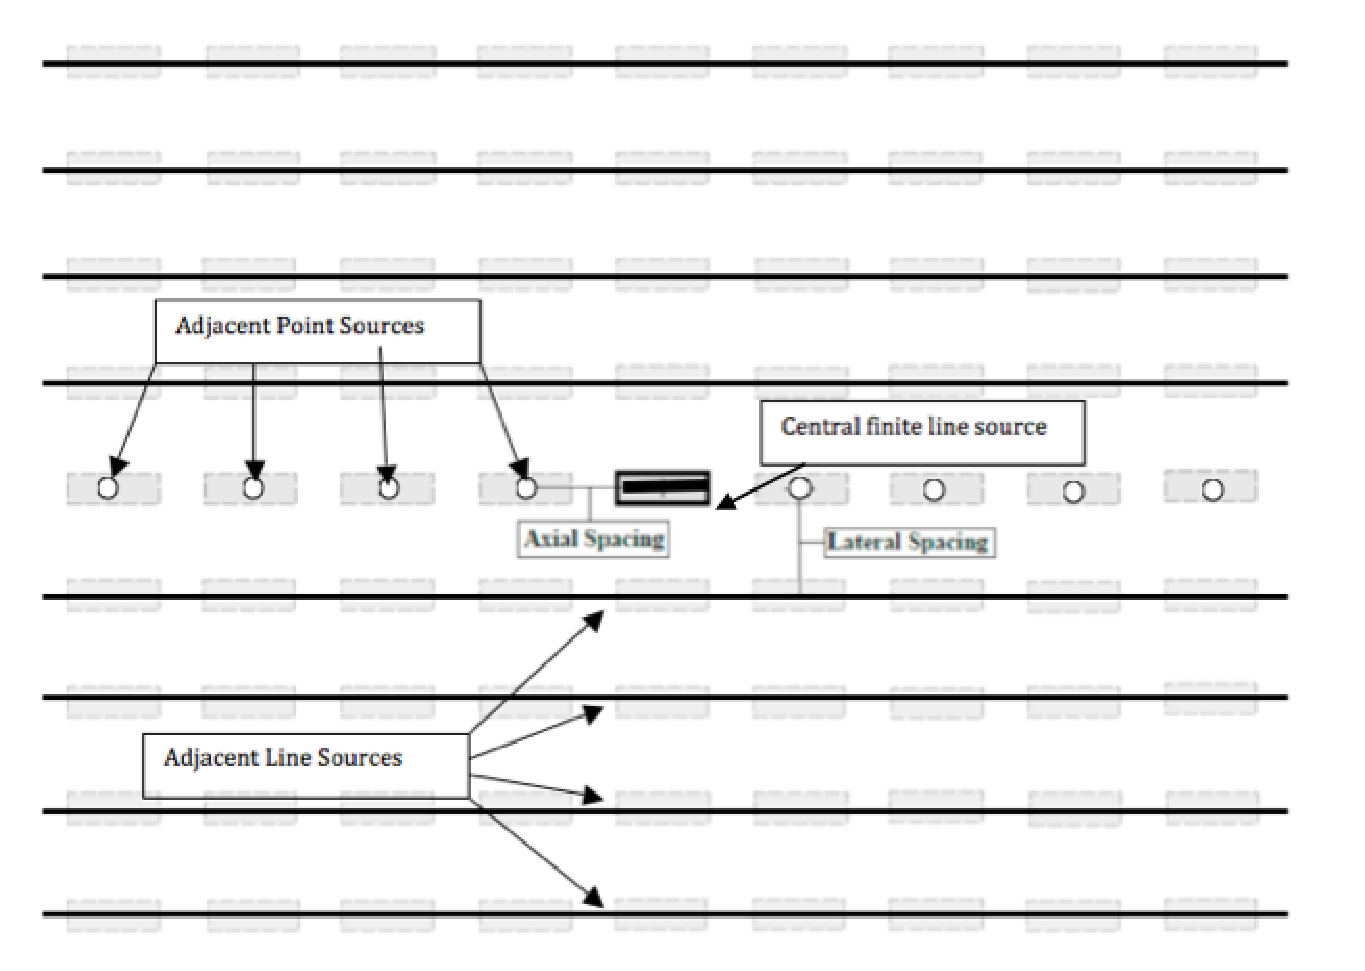
\includegraphics[width=0.5\textwidth]{./chapters/litrev/llnlConcept.eps}
  \end{center}
  \caption[LLNL analytic thermal model geometry]{The central package is represented by a finite line source, adjacent 
  packages in the central drift are represented as points, and adjacent disposal 
  tunnes are represented as infinite lines.
  \cite{greenberg_investigations_2012}.}
  \label{fig:llnl}
\end{figure}

The geometric layout of the analytic \gls{LLNL} model in Figure \ref{fig:llnl} 
shows  that the central package is represented by the finite line solution
\begin{align}
  T_{line}(t,x,y,z) &= \frac{1}{8\pi K_{th}} 
  \bigintsss_0^t\!\frac{q_L(t')}{t-t'}e^{ \frac{-\left(x^2 + z^2\right)}{4\alpha_{th} 
  (t-t')} }\nonumber\\ &\cdot\left[ \erf{\left[ \frac{1}{2} \frac{\left( y + 
  \frac{L}{2} \right)}{\sqrt{\alpha_{th}(t-t')}}  \right]} - \erf{\left[ \frac{1}{2} 
  \frac{\left( y - \frac{L}{2} \right)}{\sqrt{\alpha_{th}(t-t')}}  \right]} 
  \right]\,\mathrm{dt'},
  \label{line}
  \intertext{adjacent packages within the central tunnel are represented by the 
  point source solution }
  T_{point}(t,r) &= 
  \frac{1}{8K_{th}\sqrt{\alpha_{th}}\pi^{\frac{3}{2}}}\bigintsss_0^{-t}\!\frac{q(t')}{(t-t')^{\frac{3}{2}}}e^{\frac{-r^2}{4\alpha_{th}(t-t')}}\,\mathrm{dt'},
  \label{point}
  \intertext{and adjacent disposal tunnels are represented by infinite line 
  source solutions}
  T_{\infty line}(t,x,z) &= \frac{1}{4\pi K_{th}} 
  \bigintsss_0^t\!\frac{q_L(t')}{t-t'}e^{ \frac{-\left(x^2 + z^2\right)}{4\alpha_{th} 
  (t-t')} }
  \label{infline}
  \intertext{in infinite homogeneous media, where}
  \alpha_{th} &= ~~\mbox{thermal diffusivity } [m^2\cdot s^{-1}]\nonumber\\
  q(t) &= ~~\mbox{point heat source} [W]\nonumber\\
  \intertext{and}
  q_L(t) &= ~~\mbox{linear heat source} [W\cdot m^{-1}]\nonumber
\end{align}
Superimposed point and line source solutions allow for a notion of the 
repository layout to be modeled in the host rock.

